\chapter{Introduction: studying dark matter (DM) at different 
	scales}		
\label{chapter:1}
\epigraph{``As far as the laws of mathematics refer to reality, they are not 
certain, as far as they are certain, they do not refer to reality.''}{Albert Einstein} 
\doublespacing
% Argues why DM plays an important role for understanding cosmology


\section{Background: The successes and pitfalls of existing DM models}
Time and time again, astrophysical
observations have shown the need to include extra mass that cannot be accounted
for by light-emitting matter. So astrophysicists have named this type
of matter as dark matter (DM). In 1937, Zwicky was the first to point out the
need for DM to explain the
higher-than-expected velocity dispersion of galaxies in galaxy
clusters. Multiple subsequent observations also confirmed the finding: galaxy 
rotation
curves \citep{Rubin1970}, the ratios of the primordial elements produced in nucleosynthesis
\citep{Dar1995}, the composition of the universe e.g. $\sim 80\%$ of the mass
as DM,
from  the peak ratio of the power spectrum of 
the cosmic microwave background (CMB) \citep{Hu1997}
and galaxy cluster mergers \citep{Clowe06}, among
others. 

In additional to proving the existence, much effort has been devoted to figuring 
out the composition of DM.
Careful attempts to explain DM with known normal, baryonic matter could not match 
experimental results. 
One proposed type of candidates for DM were
failed stars or other dim MAssive Compact Halo Objects (MACHOs). 
However, the mass inferred from microlensing events of MACHOs is insufficient
to comprise of the entire mass of dark matter halos 
\citep{Alcock1996}.

Currently, the most promising types of candidates of DM are 
particles that do not belong to Standard Model (SMP,
\citealt{Bertone2005}). 
Based on this assumption, theorists have performed calculations for certain
DM particle models, based on  
the interactions of DM particles during the hot dense plasma phase of the early universe. 
 At the
beginning of this phase, the hot plasma of different particles, including DM, could participate in
the conversion to-and-from lighter particle pairs. As the universe rapidly
expanded, the plasma cooled down so that the
annihilation rate of the DM candidates became smaller than the
number density of the remaining dark matter. 
A relic population that depends on the particle mass of the DM and
the interaction cross section thus remained 
\citep{Griest1988}. They found that for the relic abundance of the particle
candidate to match the observed abundance of DM, the DM-SMP interaction
strength has to be of the same order of magnitude as
electroweak interactions. Furthermore, this type of candidate
particles would be massive and non-relativistic (or cold). 
This type of DM particle candidates is commonly referred to as the Weakly 
Interacting Massive Particle (WIMP). 

% Although many 
%  ground-based experiments have tried to detect WIMPs without success 
%  \citep{Bottino2002}, future detectors with
% directional sensitivity of DM-SM particle interaction may provide
% unambiguous detection of WIMPs \citep{Mayet2013}. 

Another implication of having a Cold Dark Matter (CDM) model can be observed
in the formed structures of our universe.  
During the primordial hot plasma phase, the kinetic energy of DM particles
determine whether they would be gravitationally bound to a overdense neighborhood. 
If the DM particles were relativistic, small overdensities below a certain scale could not have
survived as the DM constituents would escape.  By performing simulations with
a CDM model and comparing those with hot (relativistic) dark matter, 
it was shown that the CDM simulations produced more realistic (small-scale) 
structures \citep{Blumenthal1984}. 
This CDM model then forms the basis of what is commonly known as the {\it bottom-up} 
scenario of structure formation. The {\it small} DM overdensities called halos aggregated 
gas for smaller visible structures such as stars and galaxies to form first,
while larger structures such as galaxy clusters formed last from the mergers 
of smaller structures. Visible structures are therefore found to be embedded
in DM halos most of the time. 

However, the current CDM model may not tell the entire story. It is not clear
whether DM particles can interact with each other non-gravitationally.  
This is because, with a small self-interacting dark matter (SIDM) cross
section ($<$ 10 cm$^2$ g$^{-1}$, \citealt{Randall2008d}), the predictions at large scales 
are not distinguishable from those
of CDM, while the small-scale predictions ($<$ 100 Mpc) may fit the observations better
(\citealt{Spergel2000}, \citealt{Kaplinghat2013}).  

% One well-known problem of the 
% CDM model is called the 
% ``missing satellite problem''.  This describes the lower number of observed satellite 
% galaxies than are predicted in CDM simulations of galaxies (\citealt{Moore1999},
% \citealt{Klypin1999}). The discrepancy of bright satellite galaxies 
% is especially severe for our own Milky Way galaxy, which is too massive to fail
% as a host for bright satellite galaxies (\citealt{Boylan-Kolchin2011b},
% \citealt{Boylan-Kolchin2012b}). This unsolved problem is complicated by 
% observation limitations such as the incomplete depth and coverage of the
% surveys of satellite galaxies. 
The small scale discrepancy for the central density of DM halos between CDM
predictions and observations is also known as the `core or cusp' problem.   
A SIDM model predicts a flatter fall-off of the central density profiles of DM
halos as a function or radius,
resulting in `cored' profiles, while a CDM model, favors steeper fall-off of
the density, predicting `cuspy' profiles. 
For dwarf galaxies which have poor
stellar densities, the inner regions of the DM profiles were observed to have less 
steep dropoff than predicted by CDM simulations (\citealt{Rocha2013a},
\citealt{Peter2013b}, \citealt{Buckley2014}). Due to a lack of 
understanding of 
how baryonic feedback can affect the density profile of the inner regions 
dwarf galaxies, it is inconclusive which model would fit the observations of dwarf
galaxies better. In chapter 2 and 3, I will show how to constrain the SIDM interaction 
cross-section using galaxy clusters. 

\section{Techniques of inferring DM distribution - weak lensing}
A recurring theme of this work makes use of weak gravitational lensing
(thereafter weak lensing) to map
the DM distribution. Here I will explain the terminology of weak lensing
pertinent to this work by summarizing the works of \citet{Narayan1996}
and \citet{Bartelmann2001a}. Readers are encouraged to refer to the original 
sources for the full details. 
\begin{figure*}[h]
	\begin{center}
	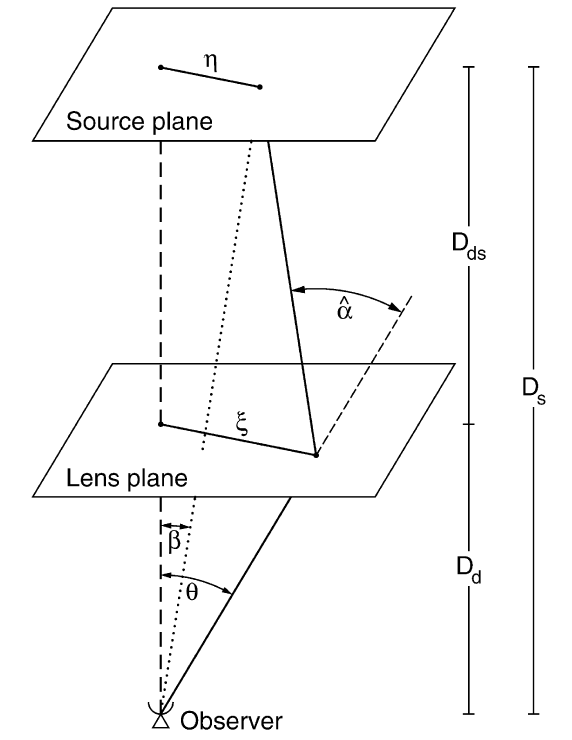
\includegraphics[width=0.5\textwidth]{lensing_figure.png}
	\caption{The sketch of a gravitational lens system created by Michael Sachs,
		under the [CC BY-SA 3.0
	(http://creativecommons.org/licenses/by-sa/3.0) or GFDL
(http://www.gnu.org/copyleft/fdl.html)] license, via Wikimedia Commons.	\label{fig:lens_sketch}
	}
	\end{center}
\end{figure*}
	From General Relativity, we know the gravity of foreground DM creates 
curvature of spacetime, the light emitted by distant galaxies
also follows paths along the curved spacetime, therefore appears {\it
lensed} by the foreground DM distribution. 
 We can write down the surface mass density of the lens
using an integral of along the line-of-sight, i.e. the redshift $z$: 
\begin{equation}
	\Sigma(\vec{\xi}) = \int \rho(\vec{\xi}, z) dz,
\end{equation}
where we use $\vec{\xi}$ to represent a two-dimensional location along the
plane of the lens.
The deflection angle of a light ray at $\vec{\xi}$ can then be represented by
accounting for the deflection at the mass element location
$\vec{\xi}'$:
\begin{equation}
	\hat{\vec{\alpha}} = \frac{4G}{c^2}\int \frac{(\vec{\xi} -
	\vec{\xi}')\Sigma(\vec{\xi}')}{|\vec{\xi} -\vec{\xi}'|} d^2\xi'
= \frac{2}{c^2}\int \vec{\nabla}_\perp \Phi dl.
\end{equation}
where $\Phi$ is the Newtonian gravitational potential.
We can illustrate the deflection in
figure \ref{fig:lens_sketch} to find the relationship between the original
source image and the deflected image:
\begin{equation}
	\vec{\eta} = \frac{D_s}{D_d}\vec{\xi} - D_{ds} \hat{\vec{\alpha}},
\end{equation}
where $D_{ds}, D_d$, and $D_s$ are the various distances indicated in 
Fig. \ref{fig:lens_sketch} respectively.
Substituting the expressions with the angular counterparts:

\begin{align}
	\vec{\beta} &= \vec{\eta} / D_s,\\
	\vec{\theta} &= \vec{\xi} / D_d, \\
	\vec{\alpha}(\vec{\theta}) &=
	\frac{D_{ds}}{D_s}\hat{\vec{\alpha}}(D_d\vec{\theta}),
\end{align}
we can read off each of these quantities (1.4 - 1.6) that appears in the lens
equation from Fig. 1.1:
\begin{equation}
	\vec{\beta} = \vec{\theta} - \vec{\alpha}.
	\label{eq:lens_equation}
\end{equation}


Furthermore, we can first define the effective lensing potential 
$\psi$ which represents a projected Newtonian potential $\Phi$ of the DM lens: 
\begin{equation}
	\psi(\vec{\theta}) = \frac{D_{ds}}{D_d D_s} \frac{2}{c^2} \int \Phi(D_d
	\vec{\theta}, z) dz.
\end{equation}
The reduced deflection angle $\alpha$ also follows:  
\begin{equation}
	\vec{\alpha} = \vec{\nabla}_\theta \psi.
\end{equation}

We can then represent the
distortions of the solid-angle of
the source galaxies in the form of a Jacobian matrix:  
\begin{align}
	\mathbf{A} \equiv \frac{\partial \vec{\beta}}{\partial \vec{\theta}} =
	\frac{\partial (\vec{\theta} - \vec{\alpha})}{\partial \vec{\theta}} =
	\left(
\begin{array}{cc}
1 - \kappa - \gamma_1 & - \gamma_2 \\
- \gamma_2 & 1 - \kappa + \gamma_1
\end{array}
\right),
\end{align}
where $\kappa$ is the dimensionless surface mass density of the lens called the
convergence, and $\gamma_1$ and $\gamma_2$ are the two components of shear.
  
This Jacobian matrix is usually expressed as,  
\begin{align}
\mathbf{A} &= (1 - \kappa)\left(
\begin{array}{cc}
1 - \frac{\gamma_1}{1 - \kappa} & - \frac{\gamma_2}{1 - \kappa} \\
- \frac{\gamma_2}{1 - \kappa} & 1 + \frac{\gamma_1}{1 - \kappa}
\end{array} 
\right) \\
& \equiv (1 - \kappa)\left(
\begin{array}{cc}
1 & 0 \\
0 & 1 
\end{array}
\right)
-
g \left(
\begin{array}{cc}
\cos 2\phi & \sin 2\phi\\
\sin 2\phi & -\cos 2\phi
\end{array}
\right). \label{eq:Jacobian_matrix}
\end{align}
The factor of 2 that exists as part of the phase of the shear, i.e. $\phi$, in
equation (\ref{eq:Jacobian_matrix}) shows 
that galaxy shapes have the properties of a spin-2 field, i.e. showing
a particular kind of rotational symmetry.  In equation 
(\ref{eq:Jacobian_matrix}), it is clear that the convergence is 
responsible for the
isotropic magnification of the light source, while the second term $g$, also
known as the reduced shear, induces changes to the ellipticities of the sources
galaxies. A definition of the convergence is that it
represents the projected surface mass density.
Since the shear is only sensitive to the gradient of the surface
mass density, shear-based techniques can reconstruct $\kappa$ up to a constant.
Physically, this constant can be thought of as a uniform sheet 
of mass in the lens plane and is commonly referred to as the mass-sheet
degeneracy. This degeneracy can be broken if information such as the 
magnification of the
source galaxies is added \citep{Narayan1996}. Another technique for breaking the 
degeneracy requires adding redshift information of individual lensed sources
\citep{Bradac2004}, but may only work for a lens with high enough mass density
within a sizable region. We focus the discussion of lensing analysis techniques
for more general cases when the signal is weak.

Analyzing data in the weak shear limit
(where $\kappa \ll 1$) allows us to approximate the induced shear as $g \approx \gamma$.
This induced shear, however, is a weak signal measured at a $\lesssim 10\%$ 
level of the observed ellipticities for galaxies lensed by galaxy clusters, and
more typically at a $\sim 1\%$ level for cosmic shear \citep{LSSTScienceCollaboration2009}.  
There are other source of contributions to the ellipticity measurements that 
can complicate the inference process. 
Galaxies are generally not round, nor can they all be described by the same 
statistical population. The intrinsic ellipticities of galaxies, also
known as shape noise, is an extra parameter that needs input during the inference.  
Other systematics that can affect ellipticity measurements include 
telescope systematics and atmospheric aberrations.
  To lower the contribution of shape noise,  
one must average the measured ellipticities of the galaxies in the 
same local area of the sky. For these reasons, the local density of source
galaxies limits the measured resolution of the DM
distribution. In chapter 3, I will show how one can
reduce the high-resolution simulated data to match
the weak-lensing resolution based on the source galaxy count.  
In chapter 4, I will elaborate further on the relationship between the 
effective lensing potential $\psi$ with the lensing observables the convergence
and shear for a joint inference.  


\section{Analyzing astronomical data with probabilistic methods}
As our generation of astrophysicists takes on new problems,
we face challenges from observations with 
low signal-to-noise or complicated models with missing variables.
Since astrophysical observations are not controlled experiments, there are limitations 
that cannot be overcome by better experimental designs nor equipment. In
Einstein's words, we need ways to deal with the uncertainties 
when applying mathematical laws to the reality. Breakthroughs in inference 
approaches for extracting scientific information are
therefore crucial for moving our field forward. 
This work describes several attempts to combine astronomical insights
with innovative modeling approaches. This section is dedicated to 
discussing the rationale behind choosing
probabilistic methods for inference, and the corresponding advantages and
disadvantages.

With a Bayesian interpretation of probability, the uncertainty of a random variable 
is expressed using its probability density function \citep{Gelman13}. This
gives a consistent representation of information for sampling and 
hierarchical modeling. Prior information of a system can also be incorporated
through weakly informative priors to achieve faster convergence of the
posterior during sampling. 
While every analysis is based on some assumptions, the
specification of the assumptions through the priors make the process 
transparent for examining the effects of the assumptions.  
A sensitivity analysis that examines how the prior choices
affect the conclusion is presented in chapter 2. 
Other diagnostics for a Bayesian analysis
can be obtained through a posterior predictive check, by generating simulated 
data from the posterior 
distribution to see if they are consistent 
with the observed data. All these diagnostics can help spot any anomaly in
the Bayesian modeling process. Another important advantage of Bayesian
methods is the ease of doing model comparisons by using the Bayes factor (see
chapter 2 for an example).
Formulating the hypothesis correctly is 
otherwise difficult via frequentist statistical tests because 
multiple tests are usually needed to compare more than one dimension of different
multivariate distributions.  

Despite all the listed advantages, Bayesian methods are known to be
computationally slow. A commonly used algorithm, the Metropolis-Hastings Monte 
Carlo Markov Chain (MCMC), only has a theoretical efficiency
(acceptance rate) of $\sim 30\%$ \citep{Roberts97}. A naive implementation of the 
powerful regression algorithm,
the Gaussian Process, also has an $O(n^3)$ computational complexity, where $n$
is the number of galaxies, due to the need
to perform expensive matrix operations. When dealing with precise data,
frequentist methods that make use of summary statistics and estimators show
comparable predictive performance and are often computationally faster. 

To model astrophysical data that has complicated dependencies and significant 
uncertainties, it is more suitable to perform a hierarchical Bayesian inference. 
In chapter 4 of this work, I have provided a graphical model 
to illustrate the hierarchical relationships between variables for the
inference of a DM mass map.
Even though no other detailed graphical model is provided, 
the same line of reasoning is still helpful for 
relating the analyses between chapter 2 and 3.  

\subsection{Reasoning using a Bayesian network}
A probabilistic graphical model (PGM), such as a Bayesian network (BN), 
provides the big picture of a comprehensive scientific analysis. 
While it is possible to come up with an
appropriate set of inference procedures without a graphical model, a graphical
model provides a succinct layout of the relationship between variables.
This is especially important when the number of variables becomes large.
The use of graphical models for inferences in robotics, natural language
processing, and medical diagnosis research have 
shown successes for modeling problems with a high number of variables 
(\citealt{Heckerman1992a}, \citealt{Koller2009}).   

Graphical models can also act as a blueprint for specifying the form of the 
 likelihood function, which is a measure of how good a statistical model fits
the observed data. A BN is represented by a directed acyclic graph (DAG). 
Each of the nodes can take one of the following forms:
\begin{itemize}
		\item a circle represents a random variable  
		\item a shaded circle represents an observed variable
		\item a dot represents a variable with fixed value.
\end{itemize}
An arrow between any two nodes indicates a statistical dependency. 
The direction of the arrow indicates the direction of influence 
of variables, although it is possible for several different graphs to represent 
the same statistical dependencies between variables 
(See Fig. \ref{fig:pgm_examples}).
The direction of the arrows can represent evidential reasoning (or explanation)
when one tries to reason from the observations to the possible causes.
Another line of reasoning, called causal reasoning, can proceed when 
one tries to predict the effects that follow a certain cause.
% All the examples here follow causal reasoning because we understand the
% deterministic physical causes, e.g. cosmology, lensing physics, etc. 
% better than the noisy observations.
The directions of the arrows are therefore not sufficient to determine how the
BN maps to a probability factorization.
The key for interpreting a graphical
model is to find out if dependency-separation exists. 
An proof of dependency-separation and an efficient algorithm for finding 
dependency-separation can be found in \cite{Meek2013} and \cite{Shachter2013}.

\begin{figure*}[h]
	\begin{center}
	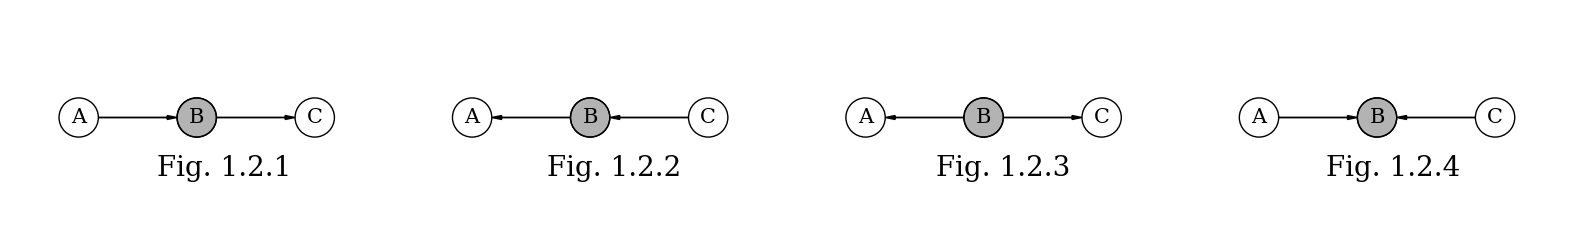
\includegraphics[width=1.\textwidth]{1pt2_pgm_examples.png}
	\caption{
		Similar looking PGMs.	Three of the four PGMs share the same factorization, 
		$P(A, B, C) = P(A | B) P(C | B) P(B)$ (Fig.
		a, b and c) while, Fig. d factors to $P(A, B, C) = P(A, C |
		B) P(B)$. In (a), observing B creates D-separation because B completely
		explains C without A. Similarly, in (b), observing B completely explains A. 
		In (c), B is a confounding factor of A and C that can induce spurious correlation,
		however, observing B, which is the cause of A and C, specifies
		its effect on both A and C, thus removing the correlation between A and C. 
		In (d), A and C both explains B. If B is explained by C
		in a certain way, then A has to explain all the effects that B
		does not explain. There is then induced correlation between A and C that
		needs to be jointly modeled. 
		\label{fig:pgm_examples}
	}
	\end{center}
\end{figure*}

The following toy example can further illustrate how the observation of variables
can affect whether a dependency-separation exists in the graph. 
During a merger between two galaxy subclusters, it is possible to observe an
offset between the DM and the density peak of the member galaxies of the
same subcluster (\citealt{Markevitch2004}, \citealt{Dawson12}, \citealt{Ng2014}), 
which we denote as  $\Delta \vec{s}$. The offset $\Delta \vec{s}$ can depend on both 
the SIDM cross-section $\sigma_{\rm SIDM}$ and other random noise from the 
merger $s_{\rm merger}$. 
Without observing any offset, $\sigma_{\rm SIDM}$ and $s_{\rm merger}$ are
statistically independent. There is no direct arrow between them, they are
d-separated. 

\begin{figure*}[h]
	\begin{center}
	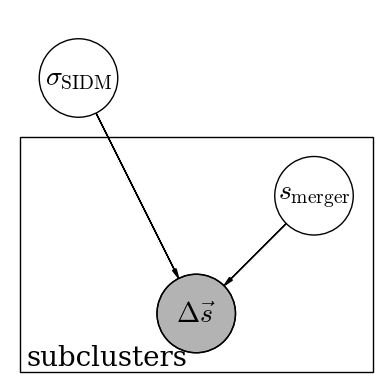
\includegraphics[width=.4\textwidth]{SIDM_pgm.png}
	\caption{PGM explaining what may give rise to a non-zero $\Delta \vec{s}$.
		The plate denotes the part of the PGM that would have different 
		$\Delta \vec{s}$ and $s_{\rm merger}$ for each galaxy cluster (denoted
		with {\it subclusters} in the figure).
		The conditional probabilities corresponding to these nodes inside the plate
		are multiplied together to form the likelihood.
		\label{fig:SIDM_inference}
	}
	\end{center}
\end{figure*}

However, once $\Delta \vec{s}$ is observed, the graph shows a v-structure that
allows the flow of influence between $\sigma_{\rm SIDM}$ and $s_{\rm
merger}$, as both of those two variables are needed to explain the observed
value of $\Delta \vec{s}$. These
statistical dependencies signal the need for a joint inference of 
$\sigma_{\rm SIDM}$ and $s_{\rm merger}$, i.e. one should {\it not} factor
$P(\sigma_{\rm SIDM}, s_{\rm merger} | \Delta
\vec{s}) \approx
P(\sigma_{\rm SIDM} |\Delta \vec{s} ) \times P(s_{\rm merger} |\Delta \vec{s})$
if the goal of the analysis is to infer $\sigma_{\rm SIDM}$.
There have been multiple examples showing how models capturing the conditional 
dependencies have superior fit to the data over models that assume
strong conditional independence (\citealt{Koller2009}). 
Realistically, $s_{\rm merger}$ can be further broken down into a
hierarchical structure that depends on the merger history of the clusters, 
and other properties of the clusters such as the makeup of the population of 
the member galaxies etc. 
Chapter 3 of this work tries to evaluate how these factors may affect $\Delta
\vec{s}$ and whether we can explain the observed values of $\Delta \vec{s}$ 
entirely without a significant $\sigma_{\rm SIDM}$. 
Another application of the graphical model can be
found in chapter 4, where there is an explicit v-structure that guides us to
jointly fit galaxy morphology properties and the Gaussian Process prior.

\begin{figure*}[h]
	\begin{center}
	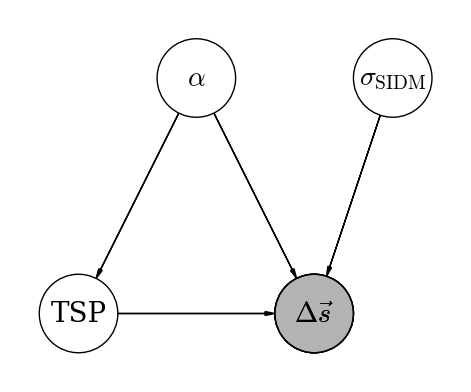
\includegraphics[width=0.4\textwidth]{confounding_alpha_PGM.png}
	\caption{
		Another toy example pertinent to the content in chapter 2. The abbreviated PGM
		shows how the projection angle of the merger axis of
		a galaxy cluster ($\alpha$)	can be an
		unobserved confounding variable that introduces additional correlation between 
		the time-since-pericenter (TSP) and  
		$\Delta \vec{s}$. Since we used a probabilistic
		Monte Carlo approach, the confounding effect is accounted for in Chapter 2.
		\label{fig:confounding_alpha}
	}
	\end{center}
\end{figure*}
There are other advanced uses of graphical models for spotting statistical
dependencies. Graphical models make it easy to spot unobserved confounding
variables that can lead to spurious correlations between other variables (See
Fig.~\ref{fig:confounding_alpha}). A graphical model also makes it clear which 
variables (i.e. the linked neighbor 
nodes) will be affected by the marginalization of a variable. 
There are explicit rules and algorithms about how to change the BN appropriately 
during variable elimination \citep{Murphy2012}. Some of these rules exploits 
the conditional independence of variables to first factor out and marginalize
some disjoint part(s) of the likelihood. After reducing the parameter space to focus
on the interested dimension, the maximization of the likelihood can be sped up.   
  
% reduce the dimensionality of
% the statistical model. Manually inserting latent variable(s) at appropriate
% location(s) of the graphical model can give an approximation of the data variables
% with decoupled statistical dependencies.  
% The approximated statistical independence 
% shows up in the covariance matrix of the variables as entries with very small
% values. This sparsity in the covariance matrix can allow faster optimization of
% the likelihood through sparse matrix inversion techniques.  

Statistical inference is, in general, at least non-deterministic polynomial (NP) 
hard. Verifying scientific hypotheses is usually even more difficult than other
prediction tasks because we cannot simply translate the problem as an 
optimization problem. The scientific hypothesis needs to be formulated 
appropriately in the statistical model. 
This is why I have employed tools such as PGMs to construct physically and 
statistically sound analyses. 

